%----------
%--- RESULTADOS

\chapter{RESULTADOS}
\thispagestyle{myheadings}

Esse capítulo busca apresentar e analisar os resultados obtidos a partir da a reestruturação do 
ETL do BDMalhas. Para isso, são comparados indicadores estruturais e de desempenho 
entre o projeto original e a implementação da solução proposta, permitindo assim analisar os ganhos 
alcançados com a solução desenvolvida.

\section{Avaliação da Manutenibilidade da Arquitetura Proposta}

Para avaliar como a reestruturação do ETL do BDMalhas impactou na manutenabilidade do sistema 
foi realizado uma contagem de metricas relacionadas à complexidade estrutural e ao esforço de 
manutenção das implementações original e proposta.

As métricas foram coletadas com base na superfície de design do SSIS, na interface web do Airflow 
e nos arquivos do novo projeto. Para a avaliação, foram considerados o número de nós, a quantidade 
de dependências entre os nós e o número de consultas SQL.


Ademais, a escolha dessas métricas se deu pelo fato de representarem os aspectos 
relacionados à complexidade estrutural e à facilidade de manutenção dos fluxos de ETL. Alem de que,
em conjunto conjunto, elas permitem avaliar o grau de modularização da solução, o nível de 
acoplamento entre as etapas, a complexidade do fluxo de execução e o esforço necessário para 
compreender, modificar e evoluir as pipelines ao longo do tempo.

No mais, as métricas coletadas estão apresentadas na Tabela \ref{tab:comparacao_manutenibilidade}, 
elaborada a partir da contagem dessas medidas em ambas as implementações.


%-------------------
%-----Tabela--------

\begin{table}[htb]
\centering
\caption{Comparação das métricas de manutenibilidade.}
\label{tab:comparacao_manutenibilidade}

\footnotesize
\renewcommand{\arraystretch}{1.2}

\newcolumntype{Y}{>{\centering\arraybackslash}X}

\begin{tabularx}{\textwidth}{|p{4.0cm}|Y|Y|Y|Y|}
\hline
\textbf{Métrica} & \textbf{NFE} & \textbf{NFCE} & \textbf{EFD} & \textbf{CTE} \\
\hline
Nós (SSIS $\rightarrow$ Airflow) &
148 $\rightarrow$ 21 (85,8\%) &
123 $\rightarrow$ 17 (86,2\%) &
222 $\rightarrow$ 76 (65,7\%) &
30 $\rightarrow$ 11 (63,3\%) \\
\hline

Dependências (SSIS $\rightarrow$ Airflow) &
124 $\rightarrow$ 26 (79,0\%) &
108 $\rightarrow$ 13 (88,0\%) &
198 $\rightarrow$ 70 (64,6\%) &
22 $\rightarrow$ 11 (50,0\%) \\
\hline

Consultas SQL (SSIS $\rightarrow$ Airflow) &
102 $\rightarrow$ 9 (91,2\%) &
84 $\rightarrow$ 6 (92,9\%) &
152 $\rightarrow$ 40 (73,7\%) &
30 $\rightarrow$ 6 (80,0\%) \\
\hline

\end{tabularx}

\vspace{0.5em}
{\small Fonte: Elaborado pelo autor, 2026}

\end{table}

A partir da leitura da Tabela \ref{tab:comparacao_manutenibilidade}, ficam evidentes os ganhos de 
manutenabilidade obtidos com a nova solução. Primeiramente, observa-se uma expressiva redução no 
número de nós em todos os quatro fluxos referentes aos diferentes documentos fiscais. Entre eles, 
os fluxos de NFCE e NFE foram os mais beneficiados, apresentando uma redução de aproximadamente 
85\% em relação à implementação original.

Essa expressiva redução deve-se, principalmente, à forma como o projeto original estava estruturado. 
Nos fluxos de NFCE e NFE do SSIS, o processo era dividido em dois grandes blocos de tarefas, 
responsáveis pela extração de notas de emitente e de destinatário. Entretanto, esses blocos eram 
praticamente idênticos, diferenciando-se apenas pelos prefixos "E" e "D" (emitente e destinatário, 
respectivamente) nos nomes das tarefas e por uma cláusula `WHERE` nas consultas SQL, utilizada para 
definir o tipo de nota fiscal a ser processada.

A existência dessa duplicação no projeto original era justificada por limitações do próprio SSIS. 
Em muitos cenários, a ferramenta não conseguia extrair, em uma única execução, todos os dados das 
notas fiscais de emitente e de destinatário devido ao elevado volume de dados. Como consequência, 
a extração frequentemente resultava em erros e perdas de conexão com o banco de dados em razão do 
longo tempo necessário para a execução das consultas.

Desse modo, com a adoção do Apache Spark e a utilização do Data Lake da UFPB como nova fonte de 
dados, optou-se por eliminar a separação entre notas de emitente e de destinatário no novo sistema 
de ETL. Essa mudança permitiu unificar o processamento em um único fluxo, reduzindo, a priori, em 
aproximadamente 50\% tanto o número de nós do workflow quanto o número de consultas SQL necessaras.

Ademais, a utilização do Data Lake e de suas consultas unificadas contribuiu significativamente 
para a redução do número de tarefas do fluxo de ETL. A Figura \ref{fig:fluxo_ssis_mult} apresenta 
um trecho do fluxo da carga de NFe, evidenciando a elevada quantidade de consultas executadas na 
implementação original. Com a adoção do esquema de dados disponibilizado pelo Data Lake, foi possível 
substituir essas múltiplas consultas por uma única consulta ao banco de dados, reduzindo 
significativamente tanto o número de nós da aplicação quanto o de consultas, assim, simplificando o 
pipeline ETL como um todo.

\begin{figure*}[ht!]
    \centering
    \caption{Exemplo de fluxo SSIS que executa multiplas consultas}\label{fig:fluxo_ssis_mult}
    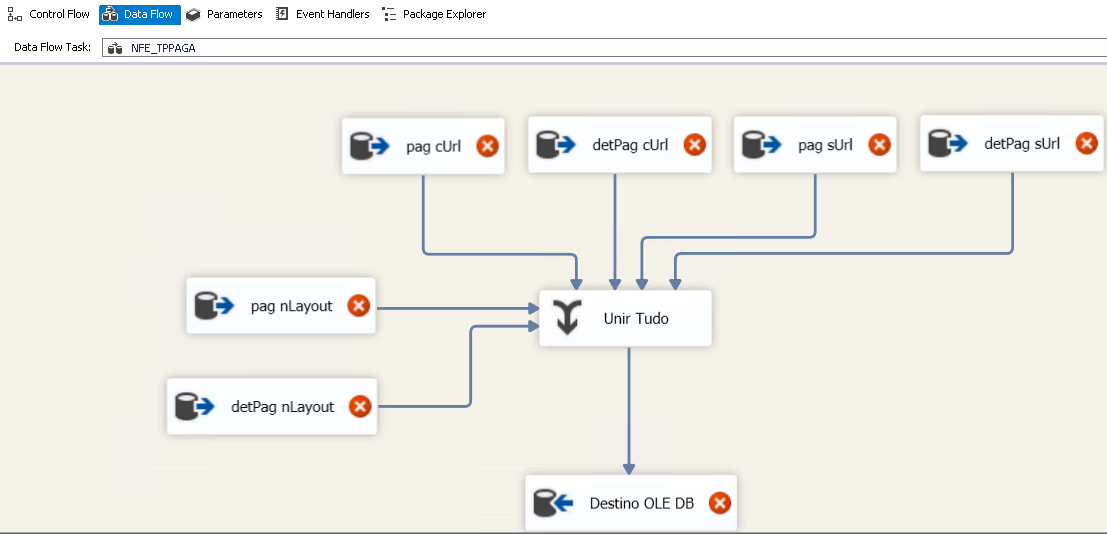
\includegraphics[width=1\textwidth]{imagens/ap_exe_task_com_multiplas_consultas.png}\\
    {\small Fonte: Elaborado pelo autor, 2026}
\end{figure*}

Já os fluxos referentes à EFD e CTE apresentaram uma redução de aproximadamente 64\% no número de 
nós. Embora esse resultado também seja expressivo, ele foi inferior ao observado nos fluxos de 
NFCE e NFE, pois essas cargas não possuíam duplicação de blocos de tarefas destinados ao processamento 
de documentos de emitente e de destinatário na implementação original.

De modo geral, a redução no número de nós desses fluxos foi resultado da junção de tarefas 
responsáveis pelas operações de registro de logs na origem e no destino com as tarefas de
extração e inserção de dados. No projeto SSIS essas tarefas são executadas de forma separada, e 
após análises, optou-se por unifica-las, reduzindo desse modo a complexidade do workflow.

A redução do número de dependecias se deu principalmente pela redução do número de nós do projeto.
Dado que, a eliminação de etapas redundantes diminuíram a quantidade de relações existentes entre as 
tarefas. 

Já as consultas SQL tiveram uma redução drástica quando comparadas ao projeto original. Como já 
mencionado anteriormente, grande parte dessa redução decorre da utilização do Data Lake como fonte 
de dados, eliminando a necessidade da execução de múltiplas consultas. Além disso, a parametrização 
permitiu o reaproveitamento de consultas comuns a diversos trechos do projeto, contribuindo ainda 
mais para a diminuição da quantidade de consultas SQL.

Como resultado, foram obtidas reduções de cerca de 90\% no número de consultas SQL dos projetos 
de NFCE e NFE. Grande parte dessa redução se deve à remoção da estratégia de notas de emitente e 
destinatário. Já os projetos de EFD e CTE também apresentaram reduções expressivas, embora menos 
acentuadas, da ordem de 80\% e 70\%, respectivamente, conforme apresentado na Tabela 
\ref{tab:comparacao_manutenibilidade}.

% Por fim temos que, a reestruturação da arquitetura do ETL promoveu uma redução significativa da 
% complexidade dos pipelines em relação à solução originalmente implementada em SSIS. Essa simplificação 
% foi possível devido à adoção de uma abordagem programática devido ao uso do Apache Airflow 
% como plataforma de orquestração e à reorganização dos dados proporcionada pelo Data Lake, 
% permitindo maior reutilização de código e redução da quantidade de componentes dos workflows.

% Nesse sentido, temos que os ganhos de manutenabilidade decorreram principallmente 
% do reaproveitamento de código SQL, lógica de processamento e regras de negócio. Adicionalmente, a 
% utilização do Data Lake da UFPB e de seu modelo de dados possibilitou a substituição de diversas 
% consultas SQL por uma única consulta, reduzindo a duplicação de codigo SQL e simplificando a
% manutenção da solução como um todo, conforme evidenciado pela Tabela 
% \ref{tab:comparacao_manutenibilidade}.


\section{Análise comparativa de desempenho}

Antes de mais nada, devemos reiterar que a quantidade de workers do Spark influencia diretamente a 
capacidade de processamento paralelo do sistema. No contexto do ambiente avaliado, foi possível
executar até seis tasks simultaneamente, contudo esse paralelismo pode variar conforme o número 
de workers do cluster Spark e as configurações do Airflow.

\begin{grafico}[ht!]
    \centering
    \caption{Tempos de execução das cargas ETL.}\label{graf:tempo_exec}
    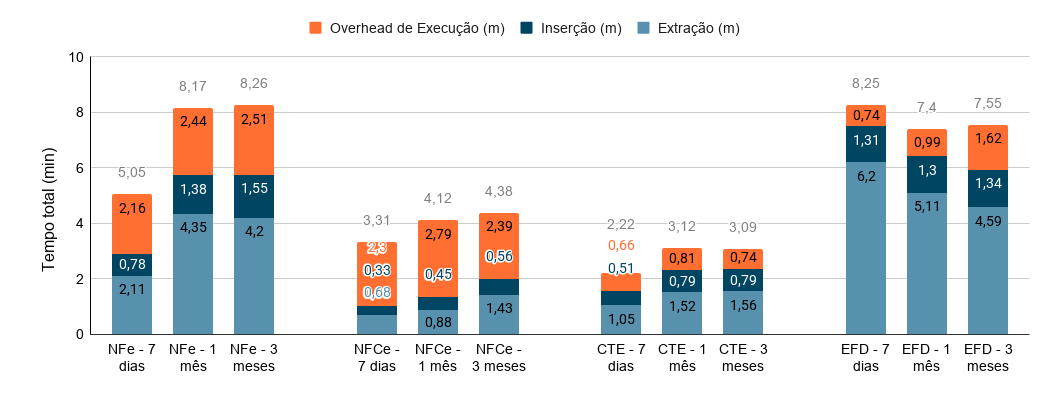
\includegraphics[width=1\textwidth]{imagens/grafico_tempo_exec}\\
    {\small Fonte: Elaborado pelo autor, 2026}
\end{grafico}

No mais, para avaliar o desempenho das cargas, foram executados experimentos 
com os quatro tipos de documentos fiscais em três intervalos temporais distintos: 
7 dias, 1 mês e 3 meses. Em cada execução, foram registrados separadamente os tempos de 
extração, inserção, overhead de execução e o tempo total da execução, permitindo uma 
análise detalhada do comportamento de cada etapa. Os resultados são apresentados 
no Gráfico \ref{graf:tempo_exec}.

Esses resultados foram coletados por meio de funcionalidades da biblioteca \textit{datetime} do 
Python e registrados na tabela \textit{sql\_log\_validacao}, responsável por armazenar os registros 
que permitem o acompanhamento da execução das cargas.

No geral, é perceptível que o novo projeto apresentou um bom tempo de execução, uma vez que nenhuma 
das cargas ultrapassou dez minutos. Contudo, deve-se lembrar que a execução das cargas ocorreu em um 
ambiente experimental, e os dados foram extraídos de uma réplica do Data Lake original. 
Essa réplica contém um volume de dados significativamente menor que o Data Lake original.

A partir do Gráfico \ref{graf:tempo_exec}, observa-se que, na maioria dos cenários avaliados, 
a etapa de extração dos dados foi a que demandou o maior tempo de execução. Em seguida, destaca-se o 
\textit{overhead} introduzido pelo Airflow e pelo Spark, enquanto a etapa de inserção dos dados 
apresentou, de forma consistente, os menores tempos de processamento.

O Gráfico \ref{graf:tempo_exec} tambem deixa perceptivel que a medida que o intervalo de tempo 
aumenta, ocorre um crescimento gradual do tempo de execução. Entretanto, esse crescimento 
mostrou-se aproximadamente proporcional ao volume processado, indicando um comportamento consistente 
da solução para diferentes quantidades de dados.

A única carga que não apresenta esse comportamento de crescimento gradual é a carga de EFD. Sua 
execução para um período de 7 dias resultou em um tempo de execução superior ao observado para os 
períodos de 1 e 3 meses. Isso provavelmente ocorreu devido à pequena quantidade de dados 
extraídos por esse fluxo. A Tabela \ref{tab:desempenho_cargas} evidencia esse comportamento, 
visto que a carga referente ao período de 3 meses extraiu apenas 2.440 registros. Considerando 
esse baixo volume de dados, é esperado que ocorram pequenas discrepâncias nos tempos de execução.

Também deve ser mencionado que a carga de EFD apresentou o maior tempo de extração, mesmo sendo a 
que extraiu a menor quantidade de registros entre todas as cargas. Isso ocorre por ela possuir o 
maior número de tarefas (nós), totalizando 76, conforme evidenciado na Tabela 
\ref{tab:comparacao_manutenibilidade}.

Outra coisa que podemos relatar a partir dos dados é que o tempo de \textit{overhead} se mantém
relativamente constante, variando pouco no contexto dos diferentes intervalos de tempo do mesmo 
documento fiscal. Isso se deve principalmente a como o fluxo dos pipelines dos documentos fiscais
estão organizados, ao número de tasks e ao número de tasks executadas em paralelo. Tanto é que
pipelines semelhantes, como os de NFE e NFCE, apresentam tempos de \textit{overhead}
tambem semelhantes. No mais, essas semelhanças entre NFE e NFCE podem ser observadas ao 
visualizar as Figuras \ref{fig:nfe} e \ref{fig:nfce} presentes no Apêndice~\ref{apend:a}.

Por fim, observa-se que os tempos de inserção permaneceram baixos em todos os fluxos avaliados, 
apresentando pouca variação mesmo com o aumento do período de dados processados. Enquanto o tempo 
de extração tende a crescer conforme o volume de registros, a etapa de inserção manteve-se 
relativamente estável, variando entre aproximadamente 0,33 e 1,55 minutos.

\subsection{Desempenho do projeto original}

\begin{grafico}[ht!]
    \centering
    \caption{Tempos de execução das cargas no projeto original.}\label{graf:tempo_ssis}
    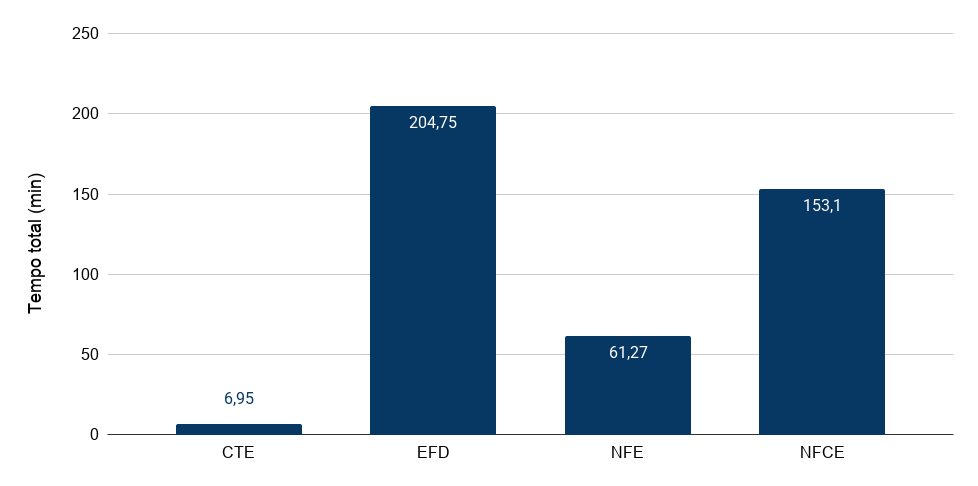
\includegraphics[width=1\textwidth]{imagens/tempos_ssis.png}\\
    {\small Fonte: Elaborado pelo autor, 2026}
\end{grafico}

Foi realizada uma execução do sistema original com o objetivo de obter os tempos de execução de cada
um dos fluxos referentes aos quatro tipos de documentos fiscais. A execução das cargas foi acionada 
pela equipe do Núcleo de Tecnologia Estratégica em Saúde (Nutes), responsável pelo desenvolvimento 
e manutenção do BDMalhas.

Desse modo, devido à dependência da equipe de membros de desenvolvimento para iniciar a execução do 
sistema baseado em SSIS, tornou-se inviável realizar sucessivas execuções das mesmas cargas para 
diferentes períodos de tempo. Por esse motivo, foi executada apenas uma carga correspondente ao 
período de janeiro a março de 2020 (3 messes).

Além disso, como o projeto de ETL original em SSIS não possui mecanismos para obter separadamente 
os tempos de extração, inserção e \textit{overhead}, foi contabilizado apenas o tempo total de 
execução.

O Gráfico \ref{graf:tempo_ssis} apresenta os tempos de execução em minutos para os quatro fluxos
de ETL, obtidos a partir da execução da solução legada no ambiente de produção. No mais, os 
dados presente no gráfico evidenciam grandes variação entre as cargas. 

A carga de CTE registrou o menor tempo de processamento, totalizando 6,95 minutos, seguida pela 
carga de NFE, com 61,27 minutos. Já as cargas de NFCE e EFD demandaram tempos significativamente 
maiores, alcançando 153,10 e 204,75 minutos, respectivamente.

Por fim, observa-se que a carga de EFD foi a que apresentou o maior tempo de execução, ultrapassando
três horas de processamento. Em contrapartida, a carga de CTE foi concluída em menos de sete minutos. 
Essa diferença evidencia que os tempos de execução variam consideravelmente entre os diferentes 
fluxos, dado que cada carga possui características próprias que influenciam diretamente sua 
duração.

\subsection{Limitações da comparação experimental}

Antes de mais nada, é importante destacar algumas limitações na comparação dos tempos de execução 
entre os dois projetos. Primeiramente, deve-se reiterar que ambos os sistemas foram executados em 
ambientes distintos. Portanto, é esperado que os resultados obtidos sejam influenciados pelas 
diferenças de infraestrutura.

Ademais, o projeto original, desenvolvido em SSIS, possui acesso direto às bases de produção do 
sistema ATF, armazenadas nos bancos Oracle e Informix, que contêm terabytes de informações fiscais. 
Em contrapartida, o projeto implementado em Airflow foi executado utilizando uma cópia do Data Lake 
original com um volume de dados significativamente menor.

Além disso, tanto as consultas SQL quanto o esquema de dados das duas versões do Data Lake ainda não
estão em sua plenitude. Em outras palavras, o esquema de dados do Data Lake ainda não representa 
integralmente o que existe nas bases de produção Oracle e Informix. Ainda há tabelas, colunas, campos,
relacionamentos e registros que precisam ser incorporados ou refinados.

Um exemplo disso é a própria carga de EFD. No projeto original, os dados a serem carregados são 
filtrados pela coluna \textit{sqcontrib}, responsável por armazenar o sequencial do contribuinte. 
Entretanto, no contexto da reestruturação, até o momento da redação deste trabalho, essa coluna 
ainda não havia sido incorporada ao Data Lake, tampouco existia um campo equivalente.

Diante desse cenário, para viabilizar a execução da carga de EFD no novo ambiente, utilizou-se a 
coluna de CNPJ do contribuinte como critério de filtragem dos dados em substituição ao 
\textit{sqcontrib}. Contudo, essa abordagem não estabelece uma correspondência exata com a 
implementação original, o que influencia os dados efetivamente carregados e, consequentemente, os 
resultados obtidos.

Ademais, diante desses fatores, é esperado que algumas das consultas disponibilizadas pela UFPB 
ainda não reflitam integralmente o comportamento das consultas implementadas no projeto original 
em SSIS, seja por diferenças no esquema de dados, seja pela ausência de determinados campos ou 
ajustes ainda pendentes. 

Dessa forma, serão necessárias futuras iterações com a equipe da UFPB para refinar o esquema de 
dados e as consultas de extração, a fim de se aproximar cada vez mais do ambiente de produção.

\section{Comparação do Projeto novo x antigo}

Tendo em vista as limitações apresentadas na subsseção anterior, podemos seguir com a 
apresentação dos resultados.

Após a execução das cargas dos quatro tipos de documentos fiscais em ambas as versões do ETL do 
BDMalhas, considerando o período compreendido entre 1º de janeiro e 31 de março de 2020, foram 
obtidos os dados referentes aos tempos de execução e às quantidades de registros extraídos e 
inseridos nos bancos de destino de ambas as aplicações. Esses resultados são apresentados na 
Tabela \ref*{tab:desempenho_cargas}, que relaciona a quantidade de registros processados com o 
tempo total de execução das cargas.


\begin{table}[H]
\centering
\caption{Desempenho das cargas executadas nas implementações avaliadas}
\label{tab:desempenho_cargas}
\begin{tabular}{lrrr}
\toprule
\textbf{Implementação} & \textbf{Registros} & \textbf{Tempo (min)} & \textbf{Registros/min} \\
\midrule
CTE -- SSIS           &    176.749 &   6,95 & 25.431,51 \\
CTE -- Nova solução   &    113.049 &   3,09 & 36.585,44 \\
\addlinespace
EFD -- SSIS           & 16.895.738 & 204,75 & 82.518,87 \\
EFD -- Nova solução   &      2.440 &   7,55 &    323,18 \\
\addlinespace
NFCE -- SSIS          &  4.253.188 & 153,10 & 27.780,46 \\
NFCE -- Nova solução  &     36.793 &   4,38 &  8.400,23 \\
\addlinespace
NFE -- SSIS           &  1.000.420 &  61,27 & 16.328,06 \\
NFE -- Nova solução   &    651.385 &   8,25 & 78.955,76 \\
\bottomrule
\end{tabular}

\caption*{\small Fonte: Elaborado pelo autor, 2026}
\end{table}

A princípio, é evidente que a quantidade de registros obtida para os mesmos documentos fiscais não 
é a mesma entre as duas implementações. Nos casos da EFD e da NFCE, as diferenças são bastante 
expressivas, chegando à ordem de milhões de registros. Isso se deve, principalmente, à utilização 
da réplica do Data Lake, que possui um volume de dados significativamente menor que o ambiente 
original.

No caso da carga de CTE, a nova solução reduziu o tempo de execução de 6,95 para 3,09 minutos, 
representando uma diminuição de 55,54\% no tempo de execução. 
Embora que, a nova solução tenha processado uma quantidade menor de registros. Contudo sua taxa 
média de processamento foi superior, passando de 25.431,51 para 36.585,44 registros por minuto, 
o que representa um aumento de 43,86\% em relação à solução baseada em SSIS.

Para a carga de EFD, a nova solução executou a carga em apenas 7,55 minutos, frente aos 204,75 
minutos da implementação em SSIS. Entretanto, essa comparação deve ser interpretada com cautela, 
pois a nova solução processou apenas 2.440 registros, enquanto a versão original carregou 16.895.738 
registros.

Na carga de NFCE, a nova solução concluiu a execução em 4,38 minutos, contra 153,10 minutos da 
implementação em SSIS. Contudo, assim como no caso da EFD, houve uma diferença significativa na 
quantidade de registros processados, impossibilitando uma comparação direta da taxa de processamento 
entre as duas implementações.

Por fim, na carga de NFE, a nova solução reduziu o tempo de execução de 61,27 para 8,25 minutos, 
correspondendo a uma redução de 86.54\% no tempo de execução. Mesmo processando uma quantidade 
menor de registros, essa carga apresentou um desempenho bem superior, atingindo
78.955,76 registros por minuto, frente aos 16.328,06 registros por minuto da solução em SSIS.
Desse modo, a taxa de registros por minuto da nova solução é aproximadamente 383,56\% 
superior à obtida pela implementação original.


\section{Comparação do Espaço de Armazenamento}

O tamanho da tabela conforme reportado pelo SQL Server.

"Os tamanhos das tabelas foram obtidos a partir das estatísticas de armazenamento disponibilizadas 
pelo SQL Server e consultadas por meio da ferramenta DBeaver."


Continua....dd